% ---------------------------------------
%
%    Beispieldiplomarbeit
%
%    - text kann gel{\"o}scht, und mit eigenen Inhalten gef{\"u}llt werden. 
%	In dieser Datei kann die gesamte Konfiguration durchgeführt werden.*
%	
%
%    *mit Ausnahme der spezifischen Optionen in natbib.cfg, die nicht von Interesse sein sollten
% ---------------------------------------

\documentclass[
    smallheadings,  % kleinere {\"U}berschriften
    twoside,        % einseitig, nur rechte seiten
    liststotoc,     % listen in inhaltsverzeichnis aufnehmen
    bibtotoc,       % literaturverzeichnis in inhltsvz. aufnehmen
    headsepline,     % trennlinie unter kopfzeile
    12pt	%Schriftgröße
    ]{scrbook}

\usepackage{a4}  %a4 Seitenformat benutzen
\usepackage[left=4cm,right=2.5cm,top=3.7cm,bottom=4cm]{geometry}
\usepackage[ngerman, english]{babel} %Verwende deutsche und amerikanische Silbentrennung
\usepackage[utf8]{inputenc} %damit k{\"o}nnen Umlaute ganz normal geschrieben werden. 

\usepackage{listings} %Fuer Codelistings

\usepackage{subfigure} %f{\"u}r mehrteilige Grafiken
\usepackage{epsfig}    %damit funktioniert das einbinden von grafiken {\"u}ber epsfig.
\usepackage{graphicx}     % zum einbinden von grafiken
\graphicspath{{grafiken}{../}{kapitel}} %da sind m{\"o}gliche bilder fuer den includegraphics-Befehl zu finden (man muss dann nicht den ganzen Pfad bei includegraphics angeben. 

\usepackage{multirow}     %fuer kompliziertere Tabellen
\usepackage{longtable}	%fuer kompliziertere Tabellen
\usepackage{rotating}	%enable landscape pages
\usepackage{framed}
\usepackage{scrpage2}     % paket f{\"u}r kopf- und fu{\ss}zeilen
\pagestyle{scrheadings}   % kopzeilenseitenstil

%\usepackage{ifpdf} %provides the switch ``ifpdf'' to determine if latex or pdflatex is executed
%see ftp://ftp.ctan.org/tex-archive/macros/latex/contrib/oberdiek/ifpdf.pdf or doc folder

\usepackage{float} % adds location parameter [H] to [htb] to force figures and tables to a location, no floating

%%%% use hyperlinks and adjust settings, see http://en.wikibooks.org/wiki/LaTeX/Hyperlinks and
% ftp://tug.ctan.org/tex-archive/macros/latex/contrib/hyperref/doc/manual.pdf
\usepackage[
a4paper=true, % a4
pdftitle={Model-Driven Game Development with Melanee}, %title to display for pdfs
pdfauthor={The Author}, %set author
%dvipdfmx, % must be used if pdf is created from the dvi file rather than by running pdflatex. Otherwise links won't work
colorlinks,% set link color for all links to black, i.e. invisible but working links
citecolor=black,%
filecolor=black,%
linkcolor=black,%
urlcolor=black, %
plainpages=false, %used with pdfpagelabels to make pdf readers show roman and arabic page numbers correctly
pdfpagelabels, %used with plainpages=false to make pdf readers show roman and arabic page numbers correctly
%pagebackref=true %false: no back-references in bibliography to citations in text
]{hyperref} %include hyperlinks for citations, urls, and references
%CAUTION: breaks color settings in dvi, pdf works fine
%%%%end: use hyperlinks

\usepackage{setspace}
\usepackage{url}          % fuer urls: schreibweise ist z.B. \url{http://www.uni-mannheim.de}
%\urlstyle{same} % makes urls in the same font as the rest of the text


%Automatisch Abkürzungsliste generieren: 2x latex, makeindex myfile.nlo -s nomencl.ist -o myfile.nls, 2x latex
\usepackage{nomencl} % um Abkürzungen aufzunehmen: \abbrev{PDA}{personal digital assistant}
\let\abbrev\nomenclature
\renewcommand{\nomname}{List of Abbreviations} %Titel der Liste hier ändern, eine von zwei Optionen nutzen
%\renewcommand{\nomname}{Abkürzungsverzeichnis} %Titel der Liste hier ändern, eine von zwei Optionen nutzen
\setlength{\nomlabelwidth}{.25\hsize}
\renewcommand{\nomlabel}[1]{#1 \dotfill}
\setlength{\nomitemsep}{-\parsep}
\makenomenclature
\newcommand{\Listofabbrev}{
\printnomenclature
\newpage
}



%Inhaltsverzeichnis
\usepackage
%[
%tocfullflat,			%alle Eintraege left-aligned, alternativ: tocflat
%tocbreakscareless		%page break between toc entry allowed
%]
{tocstyle}			%mehr Kontrolle ueber Inhaltsverzeichnis
\usetocstyle{allwithdot}	%ensure there are dots in table of contents, alternativ: noonewithdot, nopagecolumn
% docu http://www.tug.org/texlive/devsrc/Master/texmf-dist/source/latex/koma-script/tocstyle.dtx
\setcounter{secnumdepth}{3} %numbering up to fifth level in table of contents
\setcounter{tocdepth}{3} %show entries in toc up to fifth level (subsubsubsubsection)


\setlength{\parindent}{0pt}		% Einzug fuer neuen Absatz
\setlength{\parskip}\medskipamount % Abstand neuer Absatz, besser als explizite Angabe in pt

\onehalfspacing %Zeilenabstand 1,5


% kapitel{\"u}berschriften in schriftart mit serifen
\setkomafont{sectioning}{\normalfont\normalcolor\bfseries}

% gestaltung der kopfzeilen
\ohead{\pagemark}
\ifoot{}
\cfoot{}
\ofoot{} 
\cohead{}
\ihead{\headmark}
\setkomafont{pagehead}{\normalfont\bfseries}
\setkomafont{pagenumber}{\normalfont\bfseries}
\automark{section}

% ----- ende der pr{\"a}ambel ----------------------------------






\begin{document}  % dokument f{\"a}ngt an
\selectlanguage{english} %englische Silbentrennung, fuer deutsche Arbeiten: \selectlanguage{ngerman}
\frontmatter      % vorspann, kapitel r{\"o}misch nummeriert

\newgeometry{margin=3cm}
% Die Titelseite der Arbeit

\begin{titlepage}

\begin{center} % zentrieren

  % Logo der Universit{\"a}t Mannheim
  \begin{figure}[ht]
    \centering
    
\includegraphics[width=.6\textwidth]{grafiken/unilogo.png}
  \end{figure}
  
  % Vertikaler Zwischenraum
  \bigskip
  \vfill 
  %\begin{framed}
  % Titel der Arbeit und Typ der Arbeit, umrandet
    \begin{center}
     \textsc{{\LARGE Model-Driven Game Development with Melanee\\Real-Time Simulation of \\Paper Fighters\\}}
                                % Letztes \\ ist wichtig, beginnt eine neue Zeile f{\"u}r die Art der Arbeit
  
      \bigskip
  
                                % Art der Arbeit, ggf. auszutauschen gegen Seminar- oder Doktorarbeit
      \textbf{Bachelor Thesis}
    \end{center}
   % \end{framed}
    \vfill
    \vfill
  
  % Daten des Erstellers, Einreichungsdatum
  % in einer Tabelle ausgerichtet
  \begin{tabular*}{0.62\textwidth}{r@{\extracolsep{\fill}}l}
   submitted: &\ December 1st 2016\\\\
    by: &\ Johannes Michael\\
		&\ johannes.mic@gmail.com\\
    &\ born November 15th 1989\\
    &\ in Ulm\\
    \\
    Student ID Number: &\ 1388909\\
  \end{tabular*}
  \vfill
  \vfill
  
  % Unten: Kontaktdaten des Lehrstuhls f{\"u}r Softwaretechnik
  
  \rule{\textwidth}{.4pt}\\ % vertikale Linie
  University of Mannheim\\
  Chair of Software Engineering\\
  D -- 68159 Mannheim\\
  Phone: +49 621-181-3912, Fax +49 621-181-3909\\
  Internet: \url{http://swt.informatik.uni-mannheim.de}
\end{center}

\end{titlepage} % Ende des Titelblatts

%%% Local Variables: 
%%% mode: latex
%%% TeX-master: "~/Documents/DA-Vorlage/beispiel/da-beispiel"
%%% End: 
     % titelseite einbinden
\restoregeometry
\chapter{Abstract}
Due to the amount of ontological levels that Melanee offers, it is possible to illustrate and verify relationships and interaction between various entities of a system. This ability of Melanee can be used for describing different object types in a game and make it possible for a user to describe a playable level by choosing and inserting an object from a set of objects.  Model-driven game development approaches where models are prioritized to lead the game development process are becoming an arising paradigm, due to prototyping and testing being recognized as significant steps in game design. This thesis deals with the model-driven software development of levels in a two dimensional platformer game, where various entities like player characters, enemies, and level objects can be placed and modified, regarding their relationship with each other.
  % abstract einbinden
\tableofcontents            % inhaltsverzeichnis

\listoffigures              % abbildungsverzeichnis

\clearpage %tell toc that there is a pagebreak after list of tables, however the hyperlink still points to the wrong page
\addcontentsline{toc}{chapter}{\nomname} %abkuerzungen ins inhaltsverzeichnis

\Listofabbrev % liste der abkuerzungen erstellen



\mainmatter       % hauptteil, kapitel lateinisch nummeriert
%\include{kapitel/content}

\chapter{Introduction}
\section{Motivation}
Complexity in video games is dramatically increasing to provide innovative and never experienced game components to the player \cite{Blow:2004:GDH:971564.971590}. Since prototyping and testing are identified as the key stones in an iterative game development process, the automization of creating prototypes through model-driven development is proposed\cite{reyno2009automatic}. Model-driven software development has become a fundamental technique in software engineering. As it is beneficial to be able to simulate a system's model---for validation, addition, or removal of certain requirements---it is desirable to add the functionality of model simulation to a certain model. Domain-specific languages, which are based on the principles of deep modelling, are used more widely in combination with model-driven software design, due to the ability of simplefying specific parts of a system. They are preffer The release of a considerable number of sophisticated simulation software, which enables precise simulation of dynamic systems and code generation, and the recent generation of real time simulators, led model driven design approaches to become relevant in the recent past. This study discusses, whether a DSL created in Melanee can be extended to support model simulation for an external (not Java based) game engine. Therefore, we create a meta-model in Melanee, which represents our modelling language, develop a simulation in the form of a Unity application, and a Melanee plug-in, which contributes as the simulation's interface. The simulation is planed to be in form of a two dimensional platformer running on the Unity game engine.
\section{Organisation}
This study is structured as follows.
The next section (Foundations) introduces relevant foundations for this study, including fundamentals of deep modelling and model-driven software development. We will examine the current state of model-driven approaches and disscuss their role in software development nowadays. Furthermore we will focus on Melanee, a workbench for creating domain specific languages, and the frameworks forming its basis. Those are the Eclipse Modelling Framework, the Graphical Modeling Framework and the Eclipse Project, which  Melanee is built on. Last in this section we will outline the Unity game engine. Subsequently we describe \textit{Paper Figthers} (Contribution), a 2D Platformer based on a multi-level model.  We will present the components it is built on. Afterwards we introduce related works, and how the tool we develop differs from them (Related Works). Then limitations and potential extensions (Limitations and Future Work) of our tool are discussed. Finally we will disscuss the results of this work (Conclusion).

\chapter{Foundations}
\section{Model-Driven Software Development}
Due to the increasing complexity of software-based systems, the abstraction level of software has to be increased. Model-driven software development (MDSD) is a software development method which focuses on creating abstract models with a strong inner structure. Traditional ways of software development have exhibited difficulties to maintain and grant stability in their structure, due to the fact programming languages do meet their limitations very quickly, when it comes to abstraction. Models are still present in the traditional approaches for documentation purpose and to prevent inconsistency. However, its structure is hardly recognizable after the development process. The model driven approach present more efficiency, and disengages from the model based approach. Since models are constructed in a formal and abstract manner, they can abstract the software's source code completely. Hence, the inner structure of an artefact can be made compact and lucid, even for a person with no prior programming knowledge \cite{voelter2007product}.
The model is the development's primary source and is also considered being part of the final implementation. The architecture a system should have as well as the functionality it should provide can be stated in a model. Hence, there is no need for the developers to impart every detail about the software implementation to the end-user any more. Despite the fact that the software development industry is experiencing a dramatic change, of the way applications are implemented, there is no accurate definition for MDSD's specifications. However, there are still some requirements that can be implicated\cite{AtkinsonG16}. Due to the significant motivation companies, that use MDSD have, to enhance productivity, raising the return on investment of their products became a crucial factor. A company can benefit from this, whether through improving the developers' productivity in the short run, by extending a relevant software artefact's functionality, or by improving their productivity in the long run, by investing into software that is long living. Most of the companies using this approach choose the former one, and tend to enhance the functionality of an already available artefact. Hence, "the more executable functionality it can generate, the higher the productivity will be"\cite{AtkinsonG16}. The second approach is less common, although the higher the longevity of an artefact is, the more the return on investment increases. Therefore, a decreasing sensitivity for change of an institution's main artefacts is desirable. From the MDSD point of view this even forms a requirement for it.
Nowadays automated code generation enhances software quality and devlopement speed, and parts of the code can be reusable components after their definition.
Recent studies show that the influences on quality, performance, and time may depend on whether a general purpose language, or a domain-specific language was used to implement the development process. The successful application of model-driven development was significantly higher in case of a domain-specific language (DSL)\cite{whittle2014state}. Therefore, it is recommended to use MDSD with ontological modeling.\\
Due to games being software from a technical point of view, all relevant requirements and characteristics from MDSD can be applied to model-driven game development as well.
\section{Deep Modelling}
\begin{figure}
	\centering
	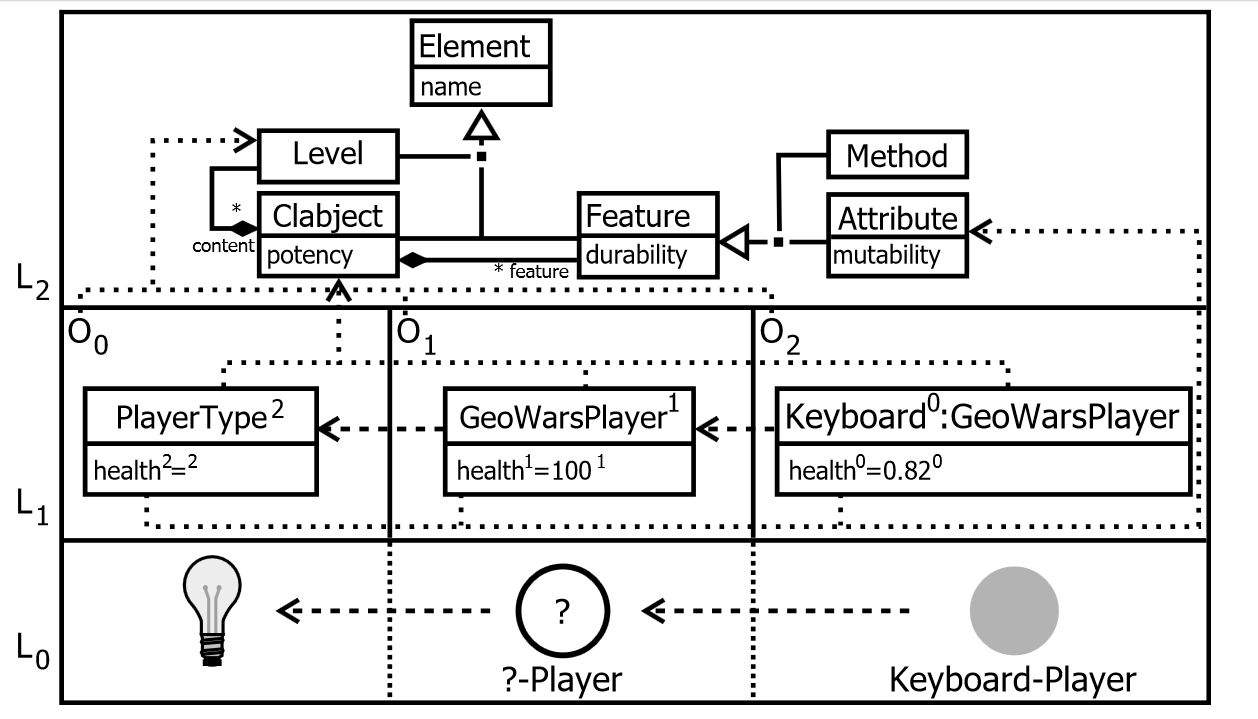
\includegraphics[scale=0.25]{grafiken/OCA.jpg} 
	\caption{The Orthogonal Classification Architecture\cite{exe2015}}
	\label{fig:1}
\end{figure}
Deep Modelling is a multi-level modelling technique developed by Atkinson and Kuehne to support model-driven software development. Conventional modelling languages and tools are based on the traditional "two levels": first the type level, in which the modelling language is described, and second the instance level containing the user model. This "two level" approach entails certain limitations, due to the lacking space for modelling instances of the user model \cite{AtkinsonG16} Deep modeling differs from this by allowing more than one logical class/instance level for a chosen domain. It supports creating models with an arbitrary number of classification levels, based on the Orthogonal Classification Architecture (OCA). Two kinds of classification relationships can be observed in [Fig. \ref{fig:1}], which illustrates an extract from the deep model of GeoWars, a multi-level model based Simulation developed by the chair of software engineering in Mannheim. The vertical dimension represents the linguistic stack, which describes all relevant concepts available in multi-level-modelling languages and entails all ontological levels. It represents the Object Management Group's Model-Driven-Architecture-Modeling-Stack\cite{AtkinsonG16}. 
The horizontal dimension describes the ontological levels.\\ L2 represents all model elements. It is referred to as the "linguistic (meta) model". The middle level L1 consists of content of the regarded domain. Thus, it holds the actual deep model and its ontological levels, O0 to O2. All model elements in L1, those in O0 excluded, each have a linguistic and a ontological type.  The lowest level (L0), consists of the real world entities, which are part of the ontological content of L1. At least three levels are typically required for model simulation and for the execution of a domain. In general the first level O0 defines the modelling language, O1 describes the model of the domain, and the third level O2 describes the instances of our domain objects, and with this the execution state of our model. Due to the fact that model elements of O1 represent instances of the types from the ontological level above and further represent types for the instances in the level underneath, they are referred to as \textit{Clabjects}, a word derived from "Class" and "Object".
Although this three level composition has become prevalent, the number of levels is unlimited in general. By deep instantiation the number of consecutive levels in which an entity from the model can be instantiated is determined. Furthermore it describes how deep a certain type can influence other types.

\section{The Eclipse Project and PDE}
The Eclipse Project is an open source software development project, which allows the development and provision of highly integrated tools.
A generic core framework for tool integration is provided, which is used by a Java development environment built. The Eclipse kernel contains a plug-in loader, which is gridded with an arbitrary amount of plug-ins. Plug-ins in the Eclipse context, are not plug-ins in the traditional way. They rather connect with a universe of plug-ins to form a running system. By being executed in an environment provided by this kernel, they can extend the environment’s services, by adding extension point to the system. Other plug-ins relying on these services can add them as an extension, to use these services. Due to the Eclipse Project's modular design, users can develop and install additional plug-ins into their workbench to extend its functionality. For developing plug-ins, the Plug-in Development Environment (PDE) is provided. It is a subproject of the Eclipse Project, which provides several tools for creating, developing, testing, debugging, building and deploying Eclipse plug-ins, fragments, features, update sites and RCP.
\section{Eclipse Modeling Framework}
The Eclipse Modeling Framework (EMF) is a code generation facility for Eclipse. It brings together the high- level engineering and modelling work and the low-level implementation programming, as two well-integrated parts of the same work. EMF provides building tools and other applications that enable the definition of a meta-metamodel from the actual model, also referred to as ecore-model. The ecore-model entails the defined classes and their names, attributes and methods. A genmodel can then be generated from the defined ecore model, which is considered to be the meta-model of our model. Afterwards the genmodel is used for describing instances of the classes from our ecore-model. Subsequently, it allows creating the domain model and the Java implementation of the meta-model, consisting the relevant instances and their attributes. Changes in a model from a higher level are forwarded to all lower level representations, due to the connection the different modelling levels have. Due to the fact that modelling concepts being directly related to their implementation, EMF allows modelling with a low cost of entry
Hence, an EMF model connects the main technologies, Java, XML, and UML, and regardless of which technology is used to define it, an EMF model is the common high-level representation that glues them all together. Therefore, it is not surprising that EMF has become a model driven software development standard, and is widely used in the industry.

\section{Graphical Modeling Framework}
The Graphical Modeling Framework(GMF) is a framework for implementing graphical editors based on EMF and GEF. For this purpose it provides certain features, like a set of reusable graphical components, a model enabling the description of diagram elements and distinguishes between the semantic (domain) and notation (diagram) elements. Moreover it provides a command infrastructure which bypasses the distinct parts of EMF's and GEF's command frameworks. Furthermore GMF is extensible and allows the implemented editors to be open and extensible.

\section{Melanee}
\begin{figure}
	\centering
	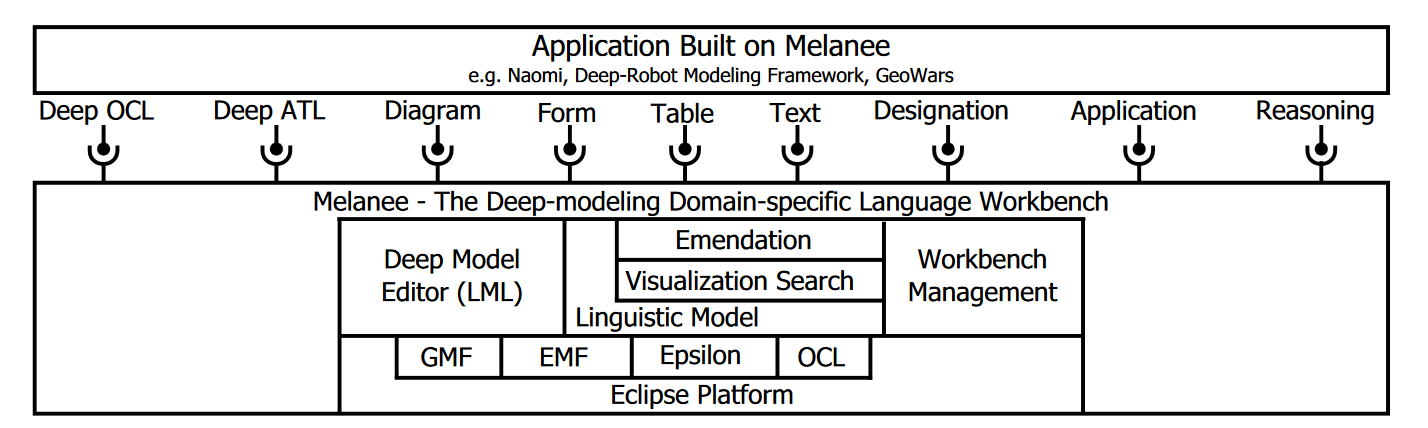
\includegraphics[width=425pt]{grafiken/extensionPoint.png}
	\caption{Melanee Architecture\cite{AtkinsonG16}}
	\label{fig:2}
\end{figure}
Melanee, developed by the Software Engineering Group at the University of Mannheim, is a workbench for creating domain-specific languages. It is based on the OCA principles and occupies an arbitrary number of ontological levels. \cite{MEL}  Most modelling tools focus on one specific format for creating domain specific languages and are regularly limited to support just two classification levels. As opposed to this Melanee supports multi-format, multi-notation domain specific modelling and due to its extendable structure the formats are limitless. The Eclipse frameworks GMF and EMF are integrated into Melanee's workbench and moreover form its foundation. This enables the use of a variety of EMF-languages and tools, which allow the deep modelling approach. Due to the fact that Melanee is an Eclipse-based application, its functionality can be extended by developing plug-ins with the Eclipse PDE. By developing extension points the contributed functionalities can be integrated into the workbench. Already available extension points, like the Deep OCL constraint language, the Deep ATL transformation language, which enables the transformation of a deep model into an ecore model, vice versa, and deep model to deep model transformation, an application language which provides altering the model environment, Reasoning, which includes model checking, and a few DSL extensions, intended to put predefined and user-defined DSLs, into the corresponding formats. Melanee is partitioned in separable components, which can be observed in [Fig. \ref{fig:2}]. The included figure shows the architecture of Melanee. It's core application offers the following features: the linguistic model, the deep model editor, visualization search algorithm, the emendation service and workbench management functionality \cite{AtkinsonG16}.

\subsection{The Level-agnostic Modeling Language and its Editor}
Creating Deep Models and defining ontological levels in it is enabled in Melanee by using the Level-agnostic Modelling language (LML). It is provided as an Eclipse plug-in, but can also be deployed as an Eclipse RCP application. %\cite{RalphDis} 
Deep instantiation is implemented in Melanee through potency attached to Clabjects (potency), Features (durability), and Attribute values (mutability)\cite{exe2015}. If an entity is defined its default potency is set to 1. When a Clabject is instantiated in a level above, its potency is decremented. If the potency of a Clabject reaches 0, it can not be instantiated in a level above.In the first level "O0" the modelling language can be specified by adding “Entities”, “Attributes”, “Methods”, “Connections/Roles”, etc. In all consecutive levels additional entities can be defined, and the entities defined in a prior level can be instantiated. 


\subsection{Extension Points and Extensions}
Since Melanee is an Eclipse based Application, the Eclipse concept of Extensions and Extension Points can be used to contribute functionality to the Melanee API. An Eclipse plug-in can use existing Extension Points as an Extension, or define Extension Points, so other plug-ins can use them as Extension. org.melanee.core.popupbutton.provider is a Melanee Extension Point of its workbench plug-in. Other Melanee pugins, which set it as an extension, can use the extension to add popup buttons to a view. 

\section{Unity and the Unity Editor}
Unity is a game engine which supports development of two- and three-dimensional video games for various platforms, like PC, Smartphones, Tablets and several gaming consoles. On Windows, it targets the Direct3D API. Due to the fact that Unity is a closed source project, the internal architecture can not be observed. However, Developers are able to use its well documented API in order to exploit the game engine. Unity Technology provides an editor, the Unity Editor, to create, run, debug and build projects.
The Unity Editor allows to build \textit{Scenes} the player is guided through. Scenes contain \textit{GameObjects}, which get functionality and shape by adding a C\#- or JS script, or other components predefined by the engine, like a variety of colliders, sprite renderer, camera components, physics components, and more to it. The Editor also provides an animation view to create and include Animations and Sprites, and an Animator which helps to manage them. The GameObject class is the Base Class for all unity entities. Various predefined child objects which are supported by Unity, like animation, physics, and a variety of colliders, are added to an instance of the GameObject. By seeding instances of this class with C\#-Scripts these child objects can be accessed and manipulated.

\subsection{Animator}

\begin{figure}
	\centering
	\includegraphics[scale=0.35]{grafiken/unityanimator.jpg}
	\caption{Unity Animator View}
	\label{fig:3}
\end{figure}

Unity consists of an animator component, which allows developers to order a set of animations for a GameObject. After adding it to the GameObjects one wants to animate, a controller can be generarted with referrences to the sprites used within it. and tells it, whether a transition shall take place. Unity also provides an editor for the animator. Its view can be observed in \ref{fig:3} which illustrates the animator of the Enemy-type "Zoys" from the Paper Fighters application. The left tab shows parameters and their state. Parameters can be triggers, boolean values, natural or real numbers, etc. The nodes represent animations, which were created in the animation editor. By clicking on them the properties are viewed in the inspector, where we can set, wheter the animation is played only once or is repetative, the time an animation takes for running once, etc. Edges between the nodes represent transitions and by opening they're properties view it can be stated, whether it depends on specific parameters, how long the transition from one animation to the other should takes, if the source animation has exit time or not. The red, blue, and green coloured states are special states, which are set into the view by default. Entry defines the starting node. If a transition is placed from it to an animation, it will turn its colour from grey to orange. In our example this can be observed by looking at the "Zoys\_fly" animation, which was grey until the transition from entry was set. By creating a transition from Any state (blue) to another state we define that the transition will take place, no matter which state the GameObject is in.
When an attack is triggered "Zoys\_attack" each will be played once, and afterwards the Animation state is set back to "Zoys\_move". \cite{UNI}
\chapter{Paper Fighters}

We develop a multi-level-model based platformer called \textit{Paper Fighters}.
The user is able to design stages with the predefined components in Melanee's Model Editor and run them directly from the model, so he can play the stages or let other people play them. The following components are relevant for playing PaperFighters: the Melanee workbench with \textit{the Paper Painter plug-in} installed, which includes the Unity Application referred to as \textit{the Paper Fighters Client} and an implemented server socket, and a meta model illustrating the game architecture referred to as textit{the Paper Model}.
To create stages the user has to run Melanee with the plugin, and instansiate a PaperLevel into the Paper Model, which then several PaperStage objects can be added into. Subsequently a PaperFighter object representing the player has to be added to each stage, so it becomes playable. Afterwards as many components, as desired, except the player object due to the fact that it is (yet) a 1 Player game.
The plug-in simulates the deep model Paper Model, a LML file created in Melanee. Afterwards the simulation is passed to the Unity application which then instantiates the simulation. As soon as the state changes the Paper Fighters application sends the current state back to the model, where the changes in the game state are instantiated and updated in a lower level of our model, so the initial level does not get affected by our simulation.\\
The position of our PaperFighter object defines the start position of the player. The Aim is to get to a door
In the following sections the three main components and their contribution to Melanee are illustrated.

\section{The Paper Fighter Client}
The Paper Fighters Client is two dimensional platformer game implemented with the Unity game engine. It represents the simulation of our game. It consists of a Scene which represents the modeled stage. Relevant GameObjects contained by the scene are the NetworkClient-Objects, whose script implements the client socket and the StageManager-Object, which is referenced by the NetworkClient.

\subsection{The StageManager and NetworkClient}
The StageManager and Networ Client are GameObjects with a scripts attached. They have no visual representation and only serve functional purpose.
The StageManager is responsible for instatiating and destroying GameObjects and keeps track of their positions. It has refferrences of all predefined GameObjects and holds classes carrying the same attributes as the ones in our model. Moreover, it holds instances of these classes. The Player-Class which keeps track of the players position, has function to manipulate its type, position, size and speed. The Enemy-Class carries the same attributes as the player but has to be distinguishable due to the player position being dependent on the players input. To instantiate the StageComponents the class Box also holds type and positioning variables, as well a fix attribute which states whether the Rigidbody2D of our component is set to isKinematic. A StageComponent's position and size depends on the following four variables: fromX, fromY, toX and toY, which define a rectangle in our scene. The differences between our from and to variables determine their size. Because the StageComponents could rotate, in case their fix attribute is set to false, the position variable is set to be the centre of the calculated rectangle. Hence, even if the component rotates, our model is not informed, but will still continuously be aware of where the centre of our component lies. In addition, the described classes each have a toString() method attached, which converts the current state of the object into a string.
The StageManager also has a SimulationToModel() function, which enables capturing the current state of the current stage in form of a string.\\
The NetworkClient is a GameObject, which holds a script for networking purposes. It creates a client socket and starts communicating with the server as soon as our application is started.
Due to both GameObjects being part of two separate threads, we included a main thread dispatcher. This script is part of our a main thread and others can use it to push their events into its queue. By this, the main thread owning the script will consume them one after another. Our StageManager has one attached to receive the clients calls, without being interrupted. However, the StageManager has to send its state back to our client socket. This implies that our networking thread likewise needs a queue.\\
This entails, that our scene will have a little delay, and the pushed events will be handled asynchronously. On the other hand the calls received from our model will be executed chronologically.

\subsection{Stage Components}
All types of Stage Components from our model, except the hinge type, are Game Objects in the Unity contex. They have a script attached which allows them to define their size, their position in the game scene, calculating the borders of the collider. Depending on the attribute "isFix: Boolean",  whether they have a Rigidbody2D components attached or not. This component makes it possible to decide, whether a Stage Component reacts to gravity and can be impacted and moved by other game objects, or whether it is simply fixed, by using Unity's physics engine. Components with this attribute set to true can be used as ground. The attached colliders vary, depending on their "type: Character" attribute the Stage Component. For the "Rectangle"-type, it is a simple BoxCollider2D, which fits the rectangle, when the size is passed to the object. The “Line”-type has an EdgeCollider2D attached. The EdgeCollider2D takes start and end point of the line as nodes and creates an edge between them. Since Unity does not provide a collider for ellipses, the “Ellipse”-type also has an EdgeCollider2D attached. The corresponding script calculates its shape’s border, sets nodes around it, and creates edges along the nodes.
The Hinge Component represents the HingeJoint2D component in unity and is a component added to a GameObject. Thus, it has to have one GameObject as a bearer. The other optional one is then referenced inside the component by the objects Rigidbody2D. By setting the hinge's anchors it can be defined whether the object is fixated by a hinge
Each Player-GameObject has a script attached, which allows him/her to move according to the player’s input and, whose methods enable modification of its attributes like walking speed, jumping height, attack cool down, and size by scripts owned by other GameObjects. One instance of the Player-type is the "BlobNinja". His abilities are double jumping, throwing shurikens, and clinging to any objects having a collider. After clinging the double jump of our ninja is reset. The idle and walking animations each consist of two pictures, while the jump consists of three animations, depending on the vertical velocity the player object has. Depending on by what the player is hit there are different animations supported by triggering one of the following methods, "HandleBurnDamage()", "HandleLightningDamage()" or "HandleDamage()".\\
The Enemy-GameObject’s script provides similar modification functionality. Furthermore, each enemy type has an additional script, where different approaches in detecting and reacting to the Player-GameObject and movement behaviour is implemented.
The "FireGhost" is able to walk left and right until he detects a player. The speed it is moving with, and the time he needs to tun around can be set by accessing the attached script. Player detection is implemented in form of a circle. If the player enters it, the enemy starts moving into his direction and attacks him as soon as he is close.
"Zoys" is a floating character. While not detecting the player, he floats left and right similar to the FireGhost. The player detection is pretty much the same as well. The main difference is that he tries to position himself above the player and attacks from there with a fast lightning bolts. His collider is only where his body is, so the cloud he is attacking from is not hittable.
The Enemy-type "KungFrog" hops around in the same manner the other two enemy-types move. as soon as he detects the player. he jumps into his direction and shoots boxing gloves out of his mouth. As soon as the player comes too close, he tries to jump over him. While he is falling, the player can receive damage from touching him.

\section{Paper Painter Plug-in}

\begin{figure}
	\centering
	\includegraphics[scale=0.9]{grafiken/meltoolbar.jpg}
	\caption{Paper Painter Toolbar}
	\label{fig:4}
\end{figure}

\begin{figure}
	\centering
	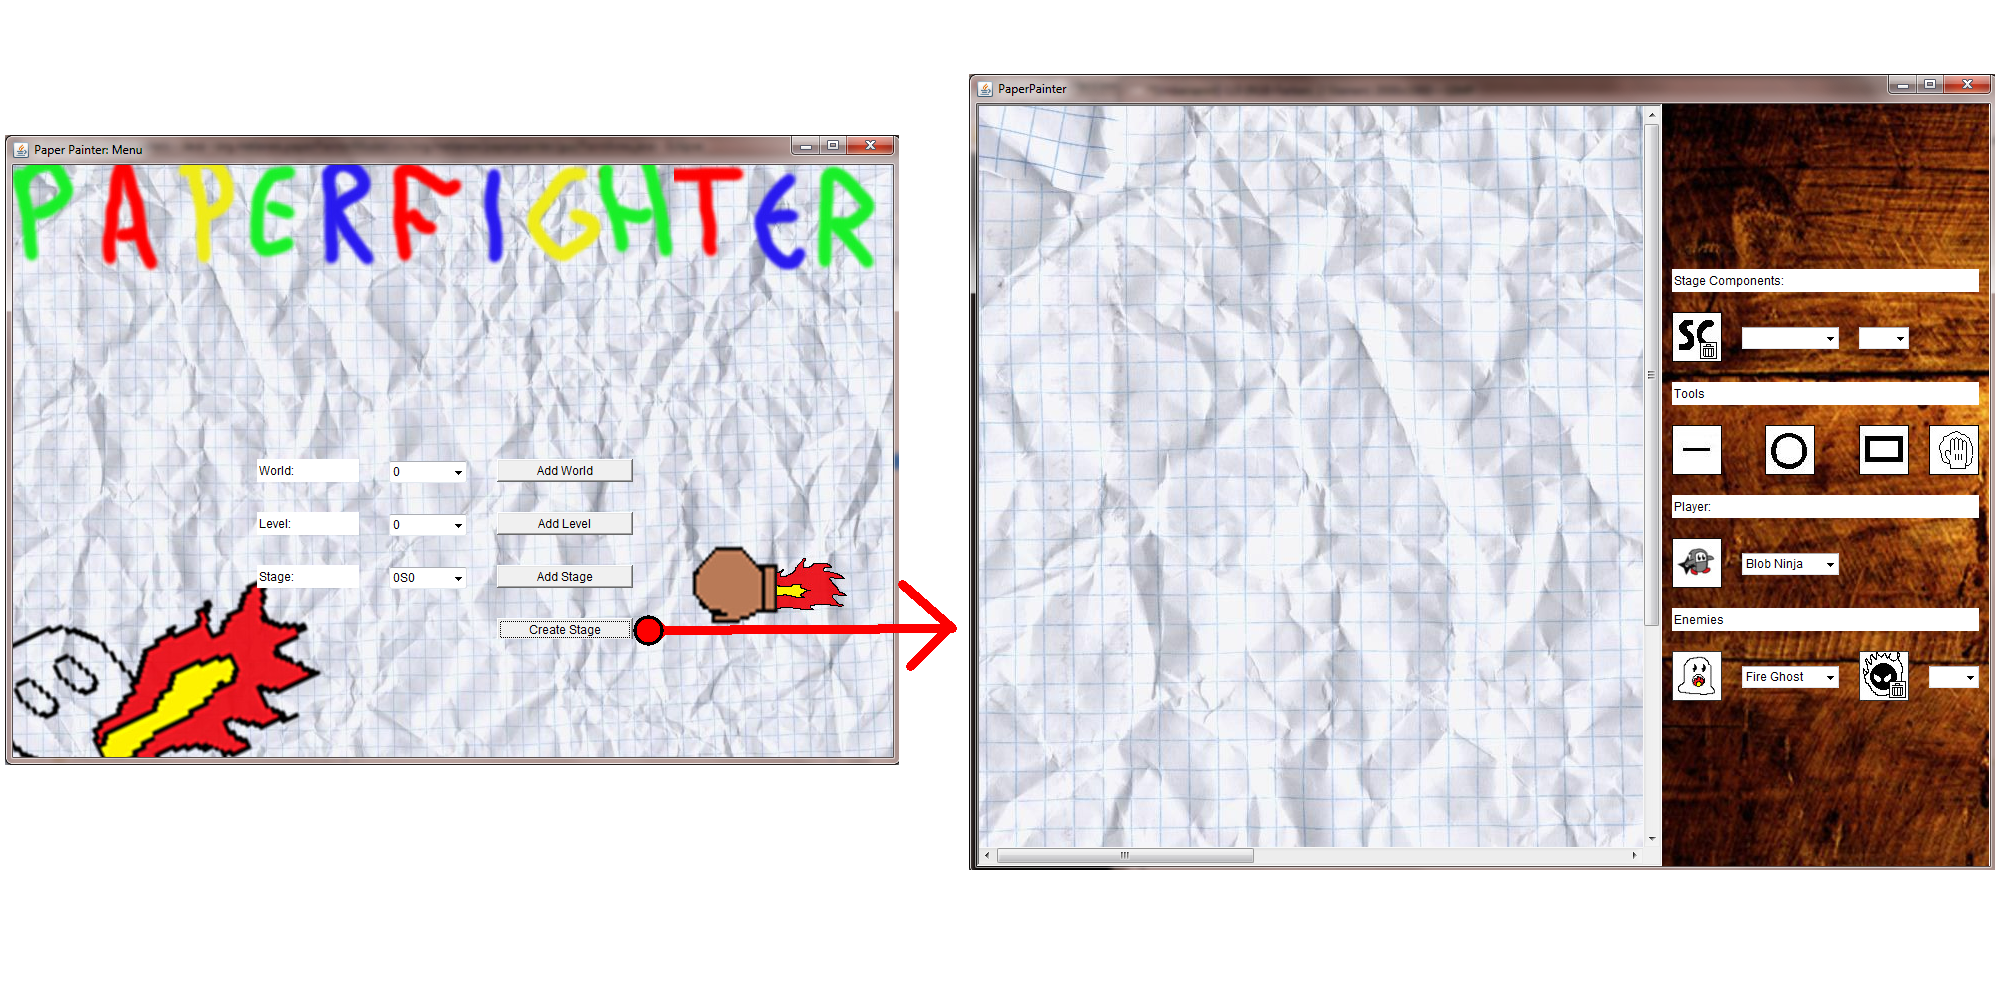
\includegraphics[scale=0.2]{grafiken/PaperPainter.png}
	\caption{Paper Painter GUI}
	\label{fig:5}
\end{figure}
We develop the Paper Painter plug-in for Melanee with the Eclipse PDE, which will be able to check the properties of an LML diagram, and to run an instance of our game if the entities' properties match our specifications. Hence, it provides modelling functionality for Paper Fighters. It uses the Melanee API to modify the deep model. The name of the created deep model must be “Paper Model“ and it has to consist of ontological levels with their names set to "O2 (Paper Model)" and "O3 (Paper Model)". As soon as these specifications are met, a Popup Bar appears in the mentioned levels with several buttons. For this purpose we extended our plug-in by the extension point org.melanee.workbench.popupbarbuttonprovider.provider. The two buttons "Let's Paint" and "Let's Play" can be observed in [Fig. \ref{fig:4}]. By pressing the "Let's Paint" button a frame implemented with the Abstract Widget Toolkit, opened, which can be observed in [Fig. \ref{fig:5}]. Within this frame instances of worlds which are a representation of a game, levels, and stages can be created. Stages are assigned to levels and levels are assigned to worlds to give a structure to one game. If the "Create Stage" button is pressed, another frame in which a painting application is implemented. With this free shapes, lines, rectangles and ellipses can be drawn. Moreover, the player-position can be set and enemies can be created and set to a desired position. The Frame instantiates them directly after they are painted holding their positions. Our Frame provides dropdown menus to select objects, declare if they are fix in the scene, and to select enemies in order to delete and reposition them. After closing the frame the objects will be passed to the corresponding stage. The "Let's Play" button creates a simulation out of our lml model and instantiates a server socket, which the simulation data is passed to. In addition it will start the Paper Fighter Client which connects with our server. Afterwards the client receives all modeled elements from the simulation as a string.
\\The plug-in is nested with classes which represent the game objects, and carry attributes corresponding to them. The classes attributes can all be modified, while the game is running via the model. The modification is then transmitted to the client, who will have to play the game with the recent modification. The Player.java, and Enemy.java classes define attributes for running speed, jumping height, size, and their position. A Box.java class defines shapes depending on its type attribute, which can be calculated inside a rectangle, like obviously rectangles, lines, and ellipses. Their position and size can also be modified during the game. Additionally, the attribute "isFix" can determine whether the object is considered as (higher) ground, or it is physically reacting to other objects, like other Box-, Enemy-, or Player-types. Furthermore, we described a FreeShape.java class which allows the modeling user to save freely painted pixels in the model, for this purpose the plug-in provides a PaperPainter.java, which is a GUI for drawing on the background and saving the drawn FreeShape- and Box-types, which both implement the interface IStageComponent.java in the PaperModel. Subsequently, we defined the class Hinge.java. It needs one and can hold up to two of type IStageComponents and has a position in the stage. When only one component is held, the component is pinned to the background at the hinges position and it can rotate around it, while when it holds two components, they are pinned to each other. By using one hinge for example on a line to pin it to the background, and another one to the line and a circle a pendulum can be modeled. The StageGoal.java class represents a way to another stage, or, if the "isLvlGoal" attribute is set, it represents the end of a level.
Representations for Stages, Levels, and Worlds are also implemented. A World contains Levels, a Level contains stages. The size of a certain Stage can be set by defining the "sizeX" and "sizeY" attributes. The background which is a A4 paper horizontally aligned is duplicated into the horizontal or vertical direction depending on the mentioned attributes. It's design was chosen to give the player the feeling to create a sketch and let it become alive. By this design different themes, like an ocean-, forest-, or volcano-theme can be retained through Levels which belong to the same world. This hierarchy is based on classical 2D platformer, which give the player the feeling of playing a story, whereby going on through the stages a kind of progress is conveyed.
\subsection{Server Socket}
As soon as the plug-in executes the unity client, it initializes a server socket and starts communicating with the client immediately. The plug-in starts three new threads, one for the server, another for receiving to messages and a third one for sending messages. Right now it is set for only one client, due to the fact that only one execution can be viewed in the model editor. Thereby the Melanee workbench will not get stopped during the communication. All classes are contained in the org.melanee.papermodel.traffic package. The code inside is provided by [\cite{SOC}]

\subsection{PaperSimulation}
The PaperSimulation.java class manages the entities of our execution model. With the "Let’s Play" button an instance of Simulation.java is instantiated and the modeled PaperLevel, its owned elements, and their properties are captured in . By getting all entities from the Paper Model our simulation creates objects from the corresponding classes contained by our plug-in.
Afterwards a server socket is initialized, and our UA is started. As soon as the UA is started, it instantiates a client socket that starts communicating with the server. When the connection is established the server sends the serialized byte stream to the client, so the created entities that match instances of our model in O1 can be created by the UA. Subsequently, the game starts sending its state back to the server as soon as something changes. The plug-in instantiates the execution state in O3, and starts updating it for each message.
The “Create Stage” button creates a new stage in the current PaperLevel context. In case, it is not the first one created, it creates a “source->next” connection to the last one created. The previous stage then becomes the source stage, and the freshly created becomes its next stage. Our simulation records the added stage and sends an update message to the UA.
Additionally, to the popup bar, our plug-in allows the user to define the position of all entities contained by a PaperStage by placing them at the desired position. As soon as the entity is placed, the position attributes are updated.
\section{Paper Model}
\begin{figure}
	\centering
	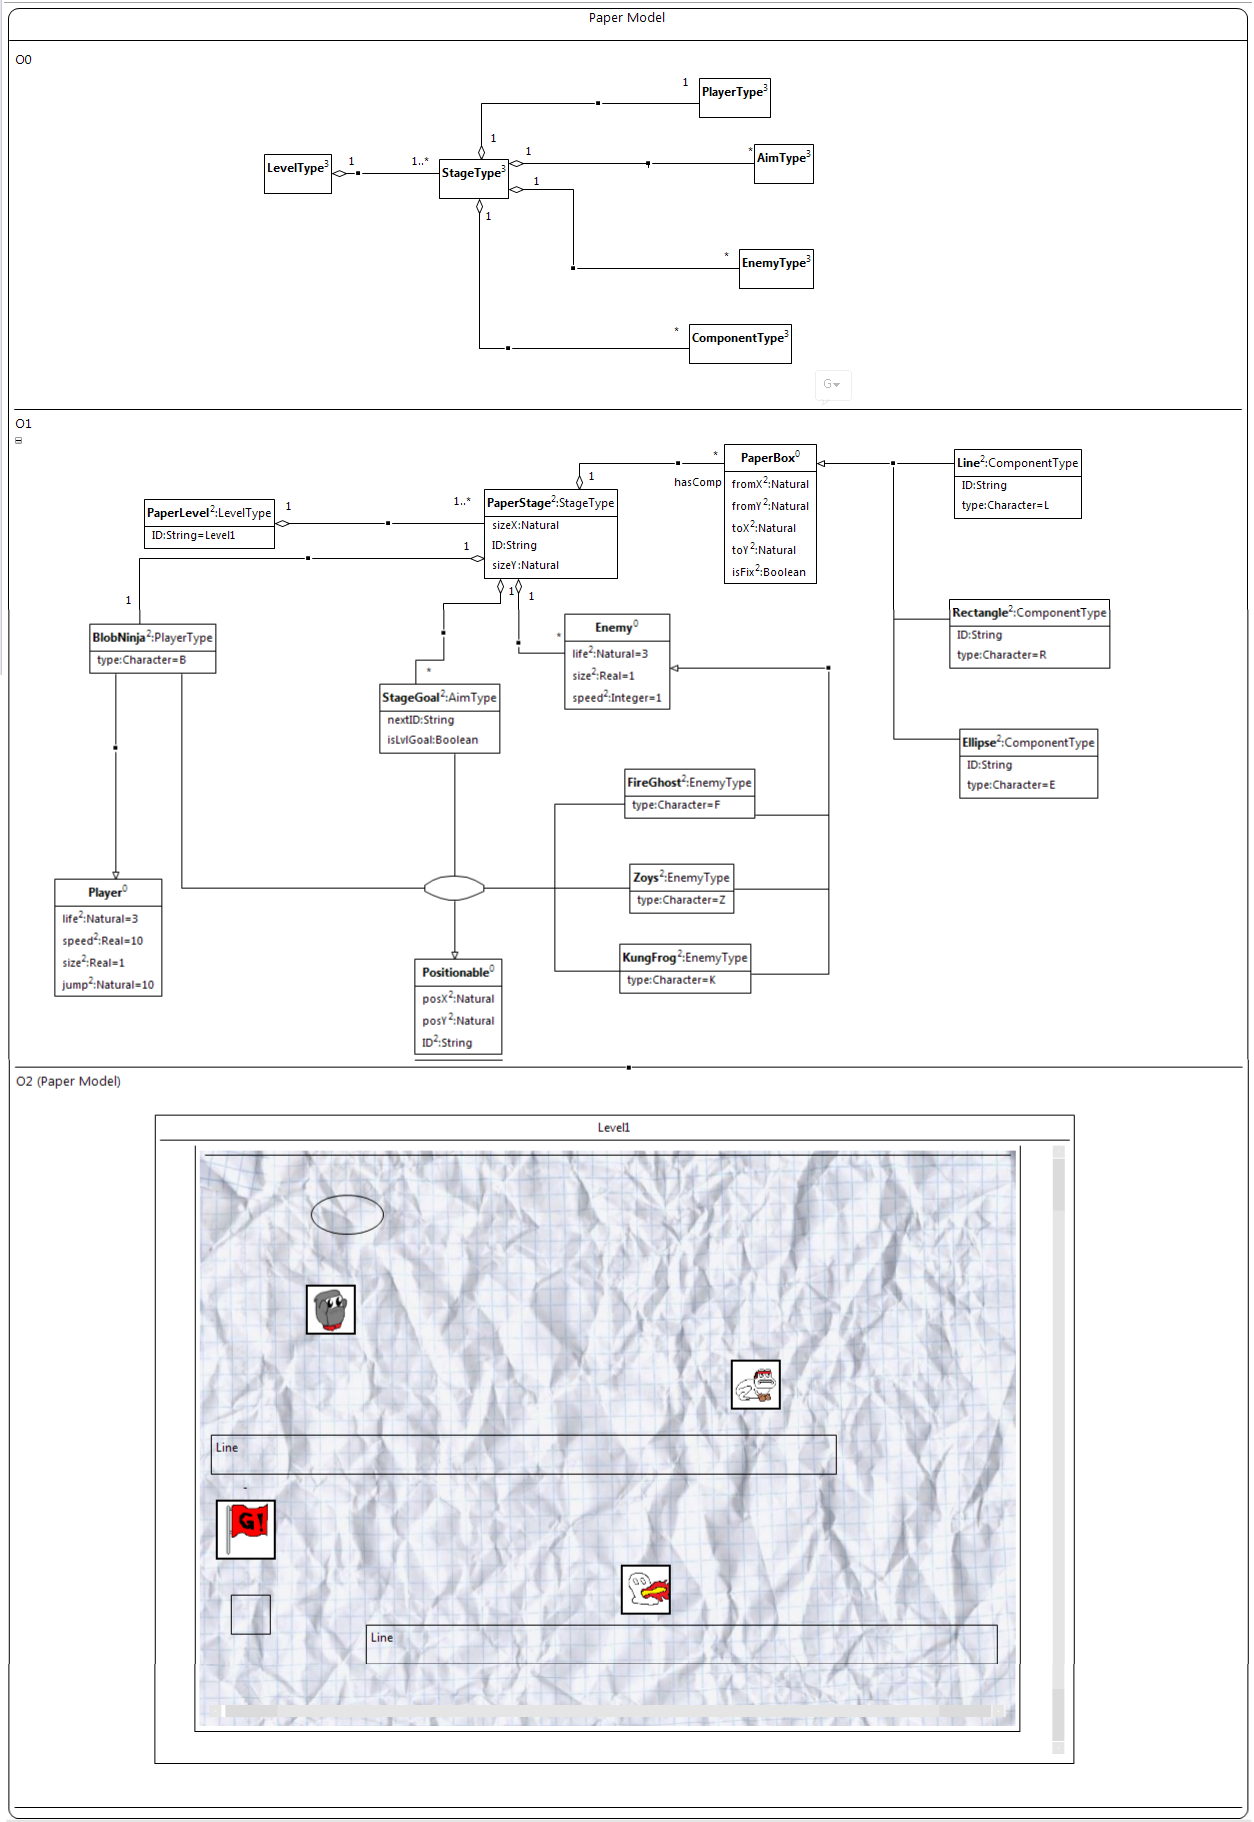
\includegraphics[scale=0.32]{grafiken/paperModel.png}
	\caption{The Paper Model}
	\label{fig:6}
\end{figure}
We create a LML diagram which represents the the model of our game by using Melanee's Model Editor. Inside the model we define the deep model \textit{Paper Model} illustrated in [Fig. \ref{fig:6}] which contains four ontological levels. "O0", defining and illustrating the modelling language, "O1", containing the actual model of our game, and "O2 (Paper Model)" which consists of an instance of the created PaperLevel.
The first level defines a modelling language for 2D platformers in general. Each game has one or more levels, where each is designed by retaining one theme to give the player the feel of a progressing story. A game level contains several stages, where one stage references other stages of the same level by adding their id to the StageGoal. By this reference it can be determined which stage can be reached from the current stage. This gives the player the feel of success, while coming closer to the last stage of the current level. Each stage contains one player, several enemies, several stage components, and one or more goals. By setting the goal’s attribute "isEnd: Boolean" the goal can be set as the end of our current level. The PlayerType is referenced by the stage, instead of the level. Hence, it is possible to set different PlayerTypes for different stages to challenge the player with different mechanics, while completing the level. The second level "O1" defines the model of Paper Fighters. It introduces its stage component types, and its enemy types. Furthermore, it shows the attributes of the stage objects. The attributes "posX: Natural" and "posY: Natural" of the differing stage objects like the player, enemies and stage goal, define their position inside the stage. In case of a PaperBox the attributes "fromX: Natural" and "fromY: Natural" define the position of the down left corner, and "toX: Natural" and "toY: Natural" define the position of the upright corner of a rectangle, in which it is instantiated. Instances of PaperFighter and PaperEnemy have additional attributes to modify their speed and size. By using Melanee’s graph-dsl plug-in we added visualization to each of the entities of "O1" instantiated in "O2", so each of their instances have a fitting visual representation in "O2 (Paper Model)".
After the initialization of the game all elements of "O2" are copied to a fourth level "O3 (Paper Model)", whose purpose is showing the execution state of the game, without having to change the initial level in "O2".
\chapter{Related Work}
Prototyping and testing became the key motivation for Model-driven development with domain specific languages. Thus, it is becoming increasingly relevant in game design and development. Whereas quite a few games allow the player to instantiate predefined object from a game model to share it with the game's community, it is surprising that real-time modelling in combination with multi-level modelling is rarely reflected upon \cite{Noah}. In this section we will show an example for a multi-level modeling based game, a number of MDGD approaches and two games sharing the benefits of model-driven level design with their players.
\section[Eine Deep-Model-Basierte Echtzeitsimulation]{Die Implementierung von GeoWars\cite{Noah}}
This thesis deals with the implementation of Geowars, a two-dimensional multi-level fighting game simulation for three players, developed by Noah Metzger from the Chair of Software Engineering at the University of Mannheim. By Using the Melanee LML editor a player can model a game level and share it through the internet. Afterwards two players can play the level against each other on one computer. The simulation feature allows modeling the current state of the played level, its objects, its players and, since the Triggerhappy-DLC also the players projectiles. Hence, it enables the simulation of a model, and real-time modification, which makes the outcome of a game more unpredictable. These principles applied to game development in general will enhance the validity of testing and prototyping.

\section{Automatic Prototyping In Model-Driven Game Development\cite{reyno2009automatic}}
This paper discusses how MDGD enhances the development process of video games by increasing the productivity and accelerating the design process. Reyno et. al. hold the belief that By abstracting the code that implements games, games are specified even more precise. To observe their statements they develop a prototype of a 2D platformer by manually programming it and compare the needed time to generating 94\% of the required code from a model with the MOFscript transformation. Instead of spending 7 days while programming it manually, they only required a few hours for generation from the model and moreover, were able to develop a second prototype by reusing the complete model from the first prototype.

\section{Super Mario Maker\cite{NIN}}
By developing a tool consisting of almost all components ever used in a two-dimensional Super Mario game and giving the opportunity to combine them with each other to the player, Nintendo produced a game that enables level modelling to its consumers. One could assume that by being the most successful platformer series ever produced the success of this project was not surprising. However, the ease of use of the level editor is also responsible for its success. The simple drag and drop function makes it easy to learn how to build stages, and if that doesn't suit the player he can simply play countless levels created from people around the world. The original use of this tool was to create Super Mario Games. This shows how the reusability of model components due to MDGD can increase the return of investment remarkably.

\section{Ultimate Chicken Horse\cite{CEG}}
Ultimate Chicken Horse is a two player 2D platformer game developed by Clever Endeavour, an indie game studio from Montreal, Canada. It combines simple level design functionality with competitive gameplay. "It's a fine balance between being an awesome level designer, and being a huge jerk"\cite{CEG}
As well as Super Mario Maker, it shows that not just the development but also the accessibility of model components to the user can be an appealing offer.
\chapter{Limitations and Future Work}
In this section we will introduce limitations and potential extensions of Paper Fighter application. First we will introduce major difficulties in this section we encountered during the development process. Subsequently, ideas that could enhance the quality of the application, like adding the concept of free shapes and hinges to the application, and enabling the levels to be accessible online.

\section{Positioning of GameObjects}
Due to not being able to access the graphical properties of our modeled elements it is not possible to set the components position by dragging and dropping them where the user wants them to be, but instead has to set the position in the properties view. Moreover, it is not possible for the user to see the actual position directly by looking at their visualisation. By adding this features the application will increase its usability and will even make it possible for children to use it.

\section{Simulation to Model}
Simulating the model does not work properly, due to difficulties of getting and modifying the graphical properties of the model elements inside of other model elements. They cannot visualize the properties of the simulated GameObjects. Furthermore, the ontological level for live execution of our simulation cannot be accessed. We will correct and extend the methods of PaperSimulation.java, contained in our plug-in in the near future. Moreover, if the connection between the server and client is lost, Melanee has to be restarted, if a new connection wants to be initialized.

\section{Parallelizing (2 Player)}
By extending the number of threads the implemented server offers it would be possible for several players to perform model simulation. The model would then be extended in its execution level O3 by an additional copy of the stage. This enables parallel model simulation from one machine. Furthermore, the game could be extended to have two or more players in one level so they can help each other and complete a stage together

\section{FreeShape and Rotation of Objects}
A GUI for creating all kind of GameObjects is also implemented and contained inside the plug-in. Giving the Visulizer Editor of Melanee the power to add free shapes which contain pixels into the model would support this feature. Other than that the visualisation of line-components inside the model would be enhanced.
Unity is able to calculate a lot of information out of its existing GameObjects and shapes. Melanee's Visualization Editor could be extended in a way that it rotates its objects. By having a rotation property, entities and instances get a new dimension in visual illustrated simulation modelling which could be useful in a different context.
Both of these extensions could be done by integrating a framework like the Batik SVG Toolkit from Apache, which not only allows displaying, generation and manipulation of SVG files, but makes these accessible for Java applications.
\chapter{Conclusion}
Paper Fighters enables multi-level modelling of two-dimensional platformer, with a set of predefined game objects. It provides the functionality of creating a stage within the LML-Editor and simulate the result.
It enables creating a complete level with several stages.
However, the plug-in does not support positioning the game objects and defining the size of the level graphically inside the model. Instead, it is only possible to set them directly in the properties view, what decreases its usability and ease of use. Moreover, the painting application contained in our plug-in is not able to assign the instantiated objects to the model, and create the simulation modelling is not possible, due to the missing conversion of the strings received from the client to the LML model entities.
Nevertheless, the result of our research is clearly the recommendation of using model-driven software development for creating complex software artefacts and systems. This extends to video games, when considering, that their complexity is dramatically increasing with upcoming technologies to provide innovative and never experienced game components to the player \cite{Blow:2004:GDH:971564.971590}. Since prototyping and testing are identified as the key stones in an iterative game development process\cite{reyno2009automatic}, the automization of creating prototypes through MDD, with real-time communication between a model and its simulation is proposed, as it enhances quality and validity of both. Especially, if a game is supposed to have a sequel or if other games of the same genre are considered in production, using MDGD is preferred. Due to the reusability of these objects the development process of future project is enhanced. All video games with respect to some exceptions, can be modeled with each game component instance considered to be an entity with specific attributes and specific relations to other entities. Hence, the model-driven approach with a DSL for developing model simulation in combination with simulation modelling for games is still recommended, due to the numerous advantages, like accelerating speed and increasing the productivity of the development effectively.

\chapter{Implementierung}

Zusammen mit dem Betreuer werden use-cases entwickelt anhand deren die
Software programmiert werden soll. Diese dienen auch als Bewertungsgrundlage.\\
\\
Die allgemein empfohlene Verzeichnisstruktur eines Projektes sieht wie folgt
aus:

\begin{itemize}
\item projektname
  \begin{itemize}
  \item bin
  \item doc
  \item lib
  \item src
  \end{itemize}
\end{itemize}

Die zu erstellende Software soll im package
de.uni\_mannheim.informatik.swt.\texttt{projektname} unter \texttt{src} liegen.\\
\\
Bei der Programmierung sollte durchgängig die englische Sprache verwendet
werden. Hierzu zählen insbesondere Kommentare im Quellcode, Namen von
Funktionen, Variable, Menüpunkte im Benutzerinterface, kurze
Hilfestellungen und Ausgaben von Programmen.\\
\\
Der Code sollte mit Hilfe von \texttt{lstinputlisting} formatiert und ausgegeben werden, wie in folgendem Beispiel:

\lstinputlisting[
  language=Java, numbers=left, stepnumber=5, firstnumber=1, breaklines=true, 
  basicstyle=\footnotesize,
  numberstyle=\tiny,
  caption={GuestbookForm.java},
  captionpos=b,
  label=GuestbookForm
]
{code/GuestbookForm.java.txt}

%\selectlanguage{english} % jetzt sprechen wir wieder englisch
%\selectlanguage{ngerman} % wenn im Inhaltsverzeichnis Appendix stehen soll, muss Engl gewaehlt sein, fuer Anhang Deutsch
%\appendix

%Bibliographie
%waehle einen der folgenden 4 Eintraege
%\bibliographystyle{literatur/natdin} %DIN Style Literaturverzeichnis, comment out pagebackref
%\bibliographystyle{literatur/IEEEtran} % IEEE Style Literaturverzeichnis
%\bibliographystyle{literatur/natdinCustomized} %DIN Style Literaturverzeichnis + Punkt hinter jeder Literaturangabe -> low level config fuer Zitate: natdin.cfg im Projektordner, comment out pagebackref
%\bibliographystyle{literatur/natdinCustomizedEnglish} %DIN Style auf Englisch getrimmt mit Punkt hinter Literaturangabe -> low lovel config fuer Zitate: natdin.cfg im Projektordner, pagebackref kann damit nicht genutzt werden
%\bibliographystyle{aer} % alternativ auch apalike, aer, apalike2... s.a. http://web.reed.edu/cis/Help/LaTeX/bibtexstyles.html
\bibliographystyle{plain} % very nice bib style
%note on aer: does not like inbook entries
%\bibliographystyle{natdin}

\bibliography{literatur/lit} %Pfad zur bib-Datei

%appendices can be defined here, the appendix structure has to be added manually to the toc (table of contents)
%\clearpage  %toc new page
%\addcontentsline{toc}{chapter}{Appendix} %add chapter to toc
%\addpart{\appendixname}
%\chapter{First class of appendices}
\section{Some appendix}

This is a sample appendix entry.

% \newpage
% \input{kapitel/methodologyQuestionMappingTable}
% 
% \input{kapitel/question_origins}
% \include{extern/fragebogenE}
% \include{extern/fragebogenD}
% 
% \input{kapitel/invitationLetters}
% 
% 
% \include{kapitel/coverageTable}

%Eidesstattliche Erklaerung
\chapter*{Eidesstattliche Erkl\"{a}rung}
\thispagestyle{empty}
Hiermit versichere ich, dass diese Abschlussarbeit von mir persönlich verfasst
ist und dass ich keinerlei fremde Hilfe in Anspruch genommen habe. Ebenso
versichere ich, dass diese Arbeit oder Teile daraus weder von mir selbst noch
von anderen als Leistungsnachweise andernorts eingereicht wurden. Wörtliche oder
sinn\-gemäße Übernahmen aus anderen Schriften und Veröffentlichungen in gedruckter
oder elektronischer Form sind gekennzeichnet. Sämtliche Sekundärliteratur und
sonstige Quellen sind nachgewiesen und in der Bibliographie aufgeführt. Das
Glei\-che gilt für graphische Darstellungen und Bilder sowie für alle
Internet-Quellen.

Ich bin ferner damit einverstanden, dass meine Arbeit zum Zwecke eines
Plagiatsabgleichs in elektronischer Form anonymisiert versendet und gespeichert
werden kann. Mir ist bekannt, dass von der Korrektur der Arbeit abgesehen werden
kann, wenn die Erklärung nicht erteilt wird.
\bigskip

\vspace{2.5cm}

Mannheim, \today \hspace{7cm} Unterschrift\\

%Abtretungs Erklaerung
\chapter*{Abtretungserkl\"arung}
\thispagestyle{empty}
Hinsichtlich meiner Studienarbeit/Bachelor-Abschlussarbeit/Diplomarbeit r\"aume ich der Universit\"at Mannheim/Lehrstuhl f{\"u}r Softwaretechnik,
Prof. Dr. Colin Atkinson, umfassende, ausschlie{\ss}liche unbefristete und
unbeschr\"ankte Nutzungsrechte an den entstandenen Arbeitsergebnissen ein.

Die Abtretung umfasst das Recht auf Nutzung der Arbeitsergebnisse in Forschung
und Lehre, das Recht der Vervielf\"altigung, Verbreitung und \"Ubersetzung sowie
das Recht zur Bearbeitung und \"Anderung inklusive Nutzung der dabei
entstehenden Ergebnisse, sowie das Recht zur Weiter\"ubertragung auf Dritte.

Solange von mir erstellte Ergebnisse in der urspr\"unglichen oder in
\"uberarbeiteter Form verwendet werden, werde ich nach Ma{\ss}gabe des Urheberrechts
als Co-Autor namentlich genannt. Eine gewerbliche Nutzung ist von dieser
Abtretung nicht mit umfasst.
\bigskip

\vspace{2.5cm}

Mannheim, \today \hspace{7cm} Unterschrift\\


\end{document}
